\documentclass{article}
\usepackage{graphicx}
\usepackage{color}
\usepackage{longtable}
\usepackage{hyperref}
\usepackage{listings}
\usepackage{draftwatermark}

\SetWatermarkText{DRAFT}
\SetWatermarkScale{5}
\graphicspath{{./images/}}
\lstset{xleftmargin=13pt}
\title {SREB Tutorial}
\begin{document}
\maketitle
Hello. This tutorial show you how to use the Stellenbosch Robotics dEvelopment Board.
\begin{figure}[h!]
	\centering
    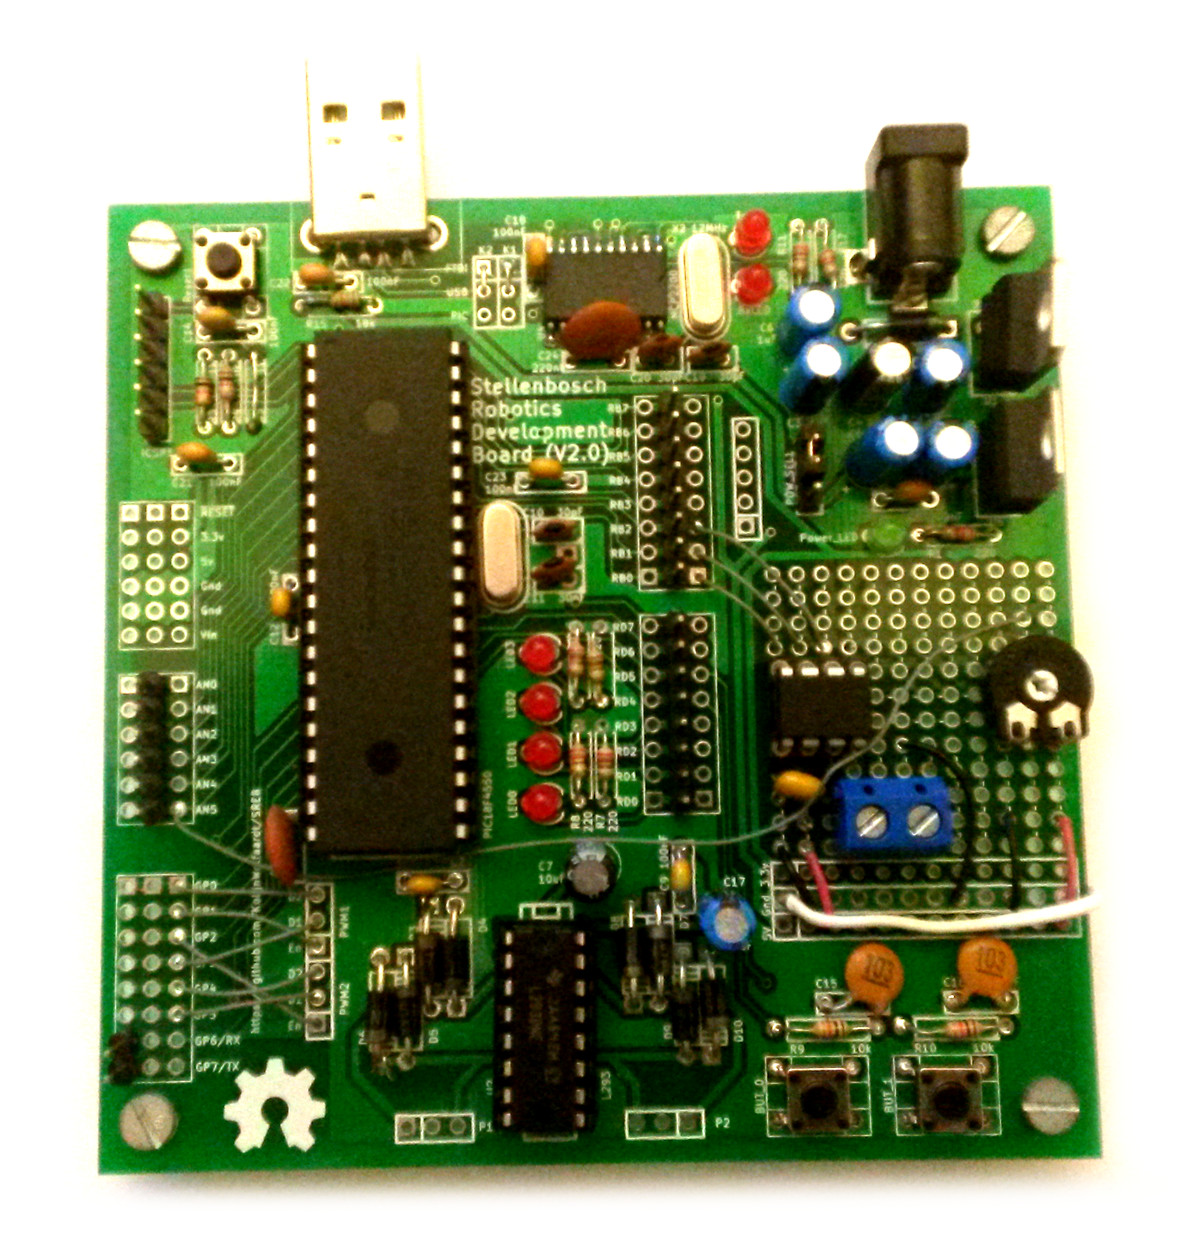
\includegraphics[scale=0.21]{full_board.jpg}
\end{figure}
\section{Hardware}
\subsection{Power Supply}
The main power supply of the board is used to convert battery power to the regulated 5v needed by the PIC. The power input is protected by a diode, to prevent reverse connection. The battery voltage needs to be above 7v to use the board. The protection diode causes a 0.7v drop, and the 7805 regulator requires at least a 6.2v input. Drawing large ammounts of  current from the board will probably cause an additional voltage drop on the battery.

The 5v source for the board is selectable between the battery and the usb. See section \ref{jumper_section} for details. The power led will turn on when the 5v is supplied to the board. The board also contains a 3.3v regulator, should you need 3.3v for any devices.

\subsection{PIC and USB}
The PIC we are using is a PIC18F4550. It is an 8-bit PIC, with a built-in USB module.

\subsection{GPIO Pins}
The GPIO (General purpose input output) pins are laid out in a simmilar fashion as an arduino, but the board is not compatible with arduino shields.

\paragraph{GPIO pins}
The two banks to the right of the PIC, RB and RD contain general purpose pins which can be used for anything. RD5 to RD0 are used for the LEDs and buttons. You can connect other devices to these lines if you want to, as long as you are aware of the possible interaction. There is another GPIO bank, to the lowwer left of the PIC, called the GP bank. The bottom 2 pins, GP6 and GP7 are used for the UART transmit and receive lines, and should not be used for any other purpose. The rest of the bank should probably be used for the motor driver, since the pwm signals are also connected there.

\paragraph{Analog and Power}
The two banks to the left of the pic are power and analog input, respectively. Below the prototyping area are 3 power rails, one for 5v, one for 3.3v and one for ground. There is also another unlabeled power rail, close to the power selection jumper. This rail provides V\_in, the input voltage after the protection diode.

\subsection{Motor Driver}
The motor driver is the L298B, and is used to control two motors. It has 6 control inputs, 3 for each motor. The motor driver receives power from the battery input, and will not work over usb power.

\subsection{Buttons and LEDS}
The buttons and LEDs are provided as a simple method of input an output. The LEDs are connected to ground via a current-limiting resistor. The buttons are connected so that they pull a line down to ground. The line is held high using a resistor. A small capacitor helps to prevent the switch bouncing.

\subsection{Jumpers And configuration}
\label{jumper_section}
\paragraph{Power selection}
There are two important configuration parts on the board. The first is the power select jumper. This allows you to select the 5v power source for the rest of the board. The input can be either the usb connector or the 5v regulated from the battery.
\begin{figure}[h!]
	\centering
    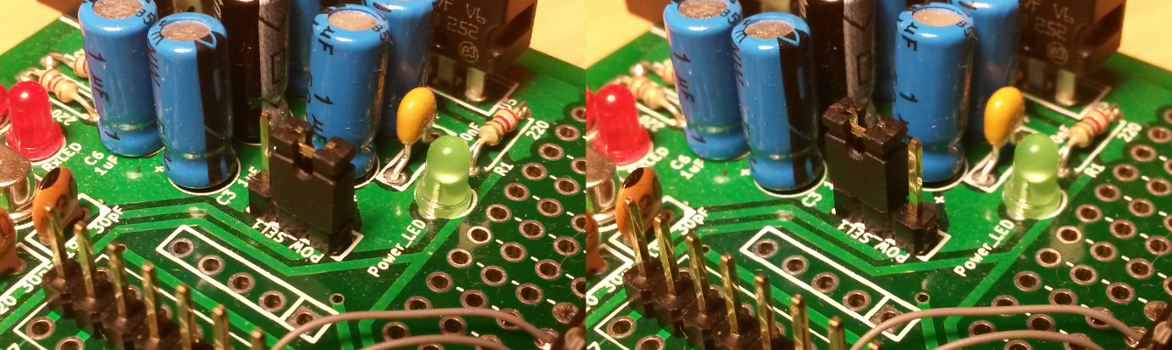
\includegraphics[scale=0.25]{power_jumper.jpg}
    \caption{Left: Power from USB. Right: Power from battery}
\end{figure}

If the usb power is selected you should not try to run high-power devices from the board, such as motors. The motor driver on the board is not powered from usb. Instead it gets power from the battery input, so it will only work when a battery is connected.


\paragraph{USB data lines}
The usb data lines (D+ and D-) can be redirected between the MCP2200 IC, and the PIC. These should normally be connected to the MCP2200, as translate UART commands from the PIC to usb. The PIC has a built in usb module which you can use if you are programming the pic using your own programmer. This can be used to emulate various usb devices, such as keyboards or sound cards. However, this is not easy. The center connection is the usb input, the top connects to the MCP2200, and the bottom to the PIC.
\begin{figure}[h!]
	\centering
    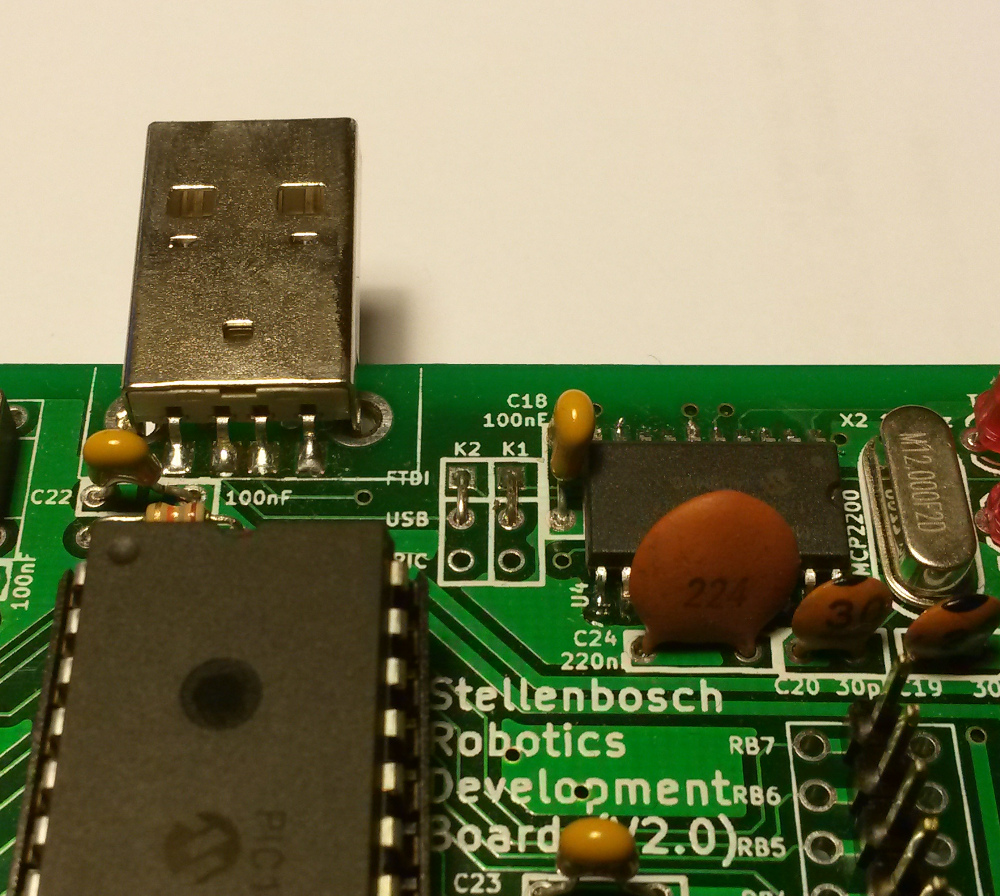
\includegraphics[scale=0.25]{usb_jumpers.jpg}
    \caption {USB connection to usb-UART IC}
\end{figure}

\section {Bootloader}
The bootloader we are using is Tinybootloader \url{http://www.etc.ugal.ro/cchiculita/software/picbootloader.htm} It was written for PICs, with the express goal of occupying very little memory in the PIC.
\paragraph{Basic conecpt}
The bootloader code is written to the PIC, and executes before the main program is run. A certain byte is sent to the PIC from the PC. If the PIC receives this before the timeout, it will start communicating with the PC and start programming. Else it will continue on to the main program.

\paragraph{Usage}
\begin{enumerate}
\item Select the hex file you want to program to the device. If you compiled using the MPLABX environment, the file might be in one of the build output folders.
\item Select the correct connection settings for the UART. The bootloader uses a 115200 baud rate.
\item Click and hold the reset button on the board. 
\item Click the \textbf{Write Flash} button, and then release the button on the board.
\item The bootloader should now program the device
\end{enumerate}
It is not neccesary to use the \textbf{CheckPIC} button before writing to the PIC. It is only used to check if the bootloader detects the PIC.

The program also features a terminal interface, allowing you to send and receive messages from the PIC. An additional feature is the graphing function, which plots the received value as a byte. This is \textit{very} helpfull when debugging sensor outputs. You can transmit the sensor value to the PC, and then whatch the output as you move the sensor. 
\paragraph{On linux}
If you want to use TinyBootloader on linux you will need to run it under \hyperref[Wine]{''http://en.wikipedia.org/wiki/Wine''}, a Linux compatibility layer for Windows. The details of installing and configuring wine will not be discussed here, and some familiarity with linux is assumed.

\begin{enumerate}
  \item To use serial ports, you need to be a member of the dialout group. This group allows you acces to serial ports and modems. To show the groups you are currently added to:

\begin{lstlisting}[language=bash,frame=single]
groups
\end{lstlisting}

If your are not in the dialout group, add yourself using

\begin{lstlisting}[language=bash,frame=single]
sudo adduser username dialout
\end{lstlisting}

To apply the changes you need to log out and log back on.

\item Next you need to find out what device the board registers as. Plug in the board, and run the following command:

\begin{lstlisting}[language=bash,frame=single]
ls /dev
\end{lstlisting}

The device should register as /dev/ttyUSB0 or /dev/ttyACM0

\item You need to tell wine about the device, so add a symbolic link called com1 to the device in the wine configuration folder. The wine configuration might be at a different location depending on your installation. You should also change the destination, the /dev/ttyACM0 part to the device the board registered as.

\begin{lstlisting}[language=bash,frame=single]
ln -s /dev/ttyACM0 ~/.wine/dosdevices/com1 
\end{lstlisting}

\item Now run TinyBootloader in wine. It will not detect the com ports automatically, you will need to enter the com port by hand. After that it should work. Note that if you unplug and replug the board, you will need to restart TinyBootloader.
\end{enumerate}

\section{Writing Code}
\subsection{MPLABX IDE}
The IDE we are using is MPLABX, which is supplied by Microchip. There is an accompaning compiler for the PIC, the XC8 compiler. These can be downloaded from the microchip site, and both work for windows and linux.

\subsection{Skeleton code}
\paragraph{Microcontroller concept:Interrupts}
A normal computer can perform more than one task at once. This is because the operating system divids computing time between different tasks. A microcontroller can also have several functions to perform, but normally does not have an operating system to organise time. Instead, the microcontroller uses interrupts. An interrupt is an event that occurs, which forces the processor to give time to another function.  

Physically an interrupt is usually implemented as a line going from an interrupt source, such as a peripheral, to the interrupt manager. When the interrupt occurs a flag is set. The processor jumps to a different place in program memory. The interrupt flag has to be cleared before the interrupt can happen again.

The implementation of interrupts vary between processors. They can usually be enbaled or disabled, and given different priorities. Some devices have an interrupt table, which determines which address to jump to depening on the interrupt. Other devices only have one address, and it is up to the programmer to handle differnet interrupts.

\paragraph{Program Flow}
A microcontroller will usually have two different sections: An initialization section, where hardware is configured and variables are set, and an endless loop, where the microcontroller reacts on inputs.

Interrupts can be used to react to several inputs, such as received messages or button presses. It is usually a good ideal to keep your interrupt code as short as possible, and then return to the main code. In the interrupt, set a flag or store the important values, and use your main loop to process the data.


\paragraph{Coding concept: State Machines}
A state machine is a device that behaves differently depening on what state it is in. It can take several inputs, and depending on them and the current state, can decide which tate to go to next. Basically an implementation of a flow diagram.

In the microcontroller this can be used to implement the different actions of the robot. THe default state is the 'driving' state. If it receives a command, or senses a line, it can go to a different state, such as waiting, or turning.

\paragraph{Analog}
\paragraph{UART}
\paragraph{Timers}
\paragraph{PWM}
\paragraph{GPIO}

\section{Appendix: Git}
\section{Appendix: Full Schematic}
\end{document}

